% Options for packages loaded elsewhere
\PassOptionsToPackage{unicode}{hyperref}
\PassOptionsToPackage{hyphens}{url}
\documentclass[
]{article}
\usepackage{xcolor}
\usepackage{amsmath,amssymb}
\setcounter{secnumdepth}{-\maxdimen} % remove section numbering
\usepackage{iftex}
\ifPDFTeX
  \usepackage[T1]{fontenc}
  \usepackage[utf8]{inputenc}
  \usepackage{textcomp} % provide euro and other symbols
\else % if luatex or xetex
  \usepackage{unicode-math} % this also loads fontspec
  \defaultfontfeatures{Scale=MatchLowercase}
  \defaultfontfeatures[\rmfamily]{Ligatures=TeX,Scale=1}
\fi
\usepackage{lmodern}
\ifPDFTeX\else
  % xetex/luatex font selection
\fi
% Use upquote if available, for straight quotes in verbatim environments
\IfFileExists{upquote.sty}{\usepackage{upquote}}{}
\IfFileExists{microtype.sty}{% use microtype if available
  \usepackage[]{microtype}
  \UseMicrotypeSet[protrusion]{basicmath} % disable protrusion for tt fonts
}{}
\makeatletter
\@ifundefined{KOMAClassName}{% if non-KOMA class
  \IfFileExists{parskip.sty}{%
    \usepackage{parskip}
  }{% else
    \setlength{\parindent}{0pt}
    \setlength{\parskip}{6pt plus 2pt minus 1pt}}
}{% if KOMA class
  \KOMAoptions{parskip=half}}
\makeatother
\usepackage{color}
\usepackage{fancyvrb}
\newcommand{\VerbBar}{|}
\newcommand{\VERB}{\Verb[commandchars=\\\{\}]}
\DefineVerbatimEnvironment{Highlighting}{Verbatim}{commandchars=\\\{\}}
% Add ',fontsize=\small' for more characters per line
\newenvironment{Shaded}{}{}
\newcommand{\AlertTok}[1]{\textcolor[rgb]{1.00,0.00,0.00}{\textbf{#1}}}
\newcommand{\AnnotationTok}[1]{\textcolor[rgb]{0.38,0.63,0.69}{\textbf{\textit{#1}}}}
\newcommand{\AttributeTok}[1]{\textcolor[rgb]{0.49,0.56,0.16}{#1}}
\newcommand{\BaseNTok}[1]{\textcolor[rgb]{0.25,0.63,0.44}{#1}}
\newcommand{\BuiltInTok}[1]{\textcolor[rgb]{0.00,0.50,0.00}{#1}}
\newcommand{\CharTok}[1]{\textcolor[rgb]{0.25,0.44,0.63}{#1}}
\newcommand{\CommentTok}[1]{\textcolor[rgb]{0.38,0.63,0.69}{\textit{#1}}}
\newcommand{\CommentVarTok}[1]{\textcolor[rgb]{0.38,0.63,0.69}{\textbf{\textit{#1}}}}
\newcommand{\ConstantTok}[1]{\textcolor[rgb]{0.53,0.00,0.00}{#1}}
\newcommand{\ControlFlowTok}[1]{\textcolor[rgb]{0.00,0.44,0.13}{\textbf{#1}}}
\newcommand{\DataTypeTok}[1]{\textcolor[rgb]{0.56,0.13,0.00}{#1}}
\newcommand{\DecValTok}[1]{\textcolor[rgb]{0.25,0.63,0.44}{#1}}
\newcommand{\DocumentationTok}[1]{\textcolor[rgb]{0.73,0.13,0.13}{\textit{#1}}}
\newcommand{\ErrorTok}[1]{\textcolor[rgb]{1.00,0.00,0.00}{\textbf{#1}}}
\newcommand{\ExtensionTok}[1]{#1}
\newcommand{\FloatTok}[1]{\textcolor[rgb]{0.25,0.63,0.44}{#1}}
\newcommand{\FunctionTok}[1]{\textcolor[rgb]{0.02,0.16,0.49}{#1}}
\newcommand{\ImportTok}[1]{\textcolor[rgb]{0.00,0.50,0.00}{\textbf{#1}}}
\newcommand{\InformationTok}[1]{\textcolor[rgb]{0.38,0.63,0.69}{\textbf{\textit{#1}}}}
\newcommand{\KeywordTok}[1]{\textcolor[rgb]{0.00,0.44,0.13}{\textbf{#1}}}
\newcommand{\NormalTok}[1]{#1}
\newcommand{\OperatorTok}[1]{\textcolor[rgb]{0.40,0.40,0.40}{#1}}
\newcommand{\OtherTok}[1]{\textcolor[rgb]{0.00,0.44,0.13}{#1}}
\newcommand{\PreprocessorTok}[1]{\textcolor[rgb]{0.74,0.48,0.00}{#1}}
\newcommand{\RegionMarkerTok}[1]{#1}
\newcommand{\SpecialCharTok}[1]{\textcolor[rgb]{0.25,0.44,0.63}{#1}}
\newcommand{\SpecialStringTok}[1]{\textcolor[rgb]{0.73,0.40,0.53}{#1}}
\newcommand{\StringTok}[1]{\textcolor[rgb]{0.25,0.44,0.63}{#1}}
\newcommand{\VariableTok}[1]{\textcolor[rgb]{0.10,0.09,0.49}{#1}}
\newcommand{\VerbatimStringTok}[1]{\textcolor[rgb]{0.25,0.44,0.63}{#1}}
\newcommand{\WarningTok}[1]{\textcolor[rgb]{0.38,0.63,0.69}{\textbf{\textit{#1}}}}
\usepackage{graphicx}
\makeatletter
\newsavebox\pandoc@box
\newcommand*\pandocbounded[1]{% scales image to fit in text height/width
  \sbox\pandoc@box{#1}%
  \Gscale@div\@tempa{\textheight}{\dimexpr\ht\pandoc@box+\dp\pandoc@box\relax}%
  \Gscale@div\@tempb{\linewidth}{\wd\pandoc@box}%
  \ifdim\@tempb\p@<\@tempa\p@\let\@tempa\@tempb\fi% select the smaller of both
  \ifdim\@tempa\p@<\p@\scalebox{\@tempa}{\usebox\pandoc@box}%
  \else\usebox{\pandoc@box}%
  \fi%
}
% Set default figure placement to htbp
\def\fps@figure{p}
\makeatother
\setlength{\emergencystretch}{3em} % prevent overfull lines
\providecommand{\tightlist}{%
  \setlength{\itemsep}{0pt}\setlength{\parskip}{0pt}}
\usepackage{bookmark}
\IfFileExists{xurl.sty}{\usepackage{xurl}}{} % add URL line breaks if available
\urlstyle{same}
\hypersetup{
  hidelinks,
  pdfcreator={LaTeX via pandoc}}

\author{}
\date{}

\begin{document}

\section{Weekly Report}\label{weekly-report}

\subsection{What I worked on this
week}\label{what-i-worked-on-this-week}

\subsubsection{Built all programs in the project
dir}\label{built-all-programs-in-the-project-dir}

\subsubsection{Created a script to run and profile
ABINIT}\label{created-a-script-to-run-and-profile-abinit}

I created a to run and profile ABINIT, meant to be the blueprint for the
other programs

\paragraph{ABINIT profile}\label{abinit-profile}

I ran ABINIT on its 0th test case on 2 nodes with 16 MPI tasks. I set
PEAK to profile memory, BLAS, LAPACK, and FFTW.

\begin{figure}
\centering
\pandocbounded{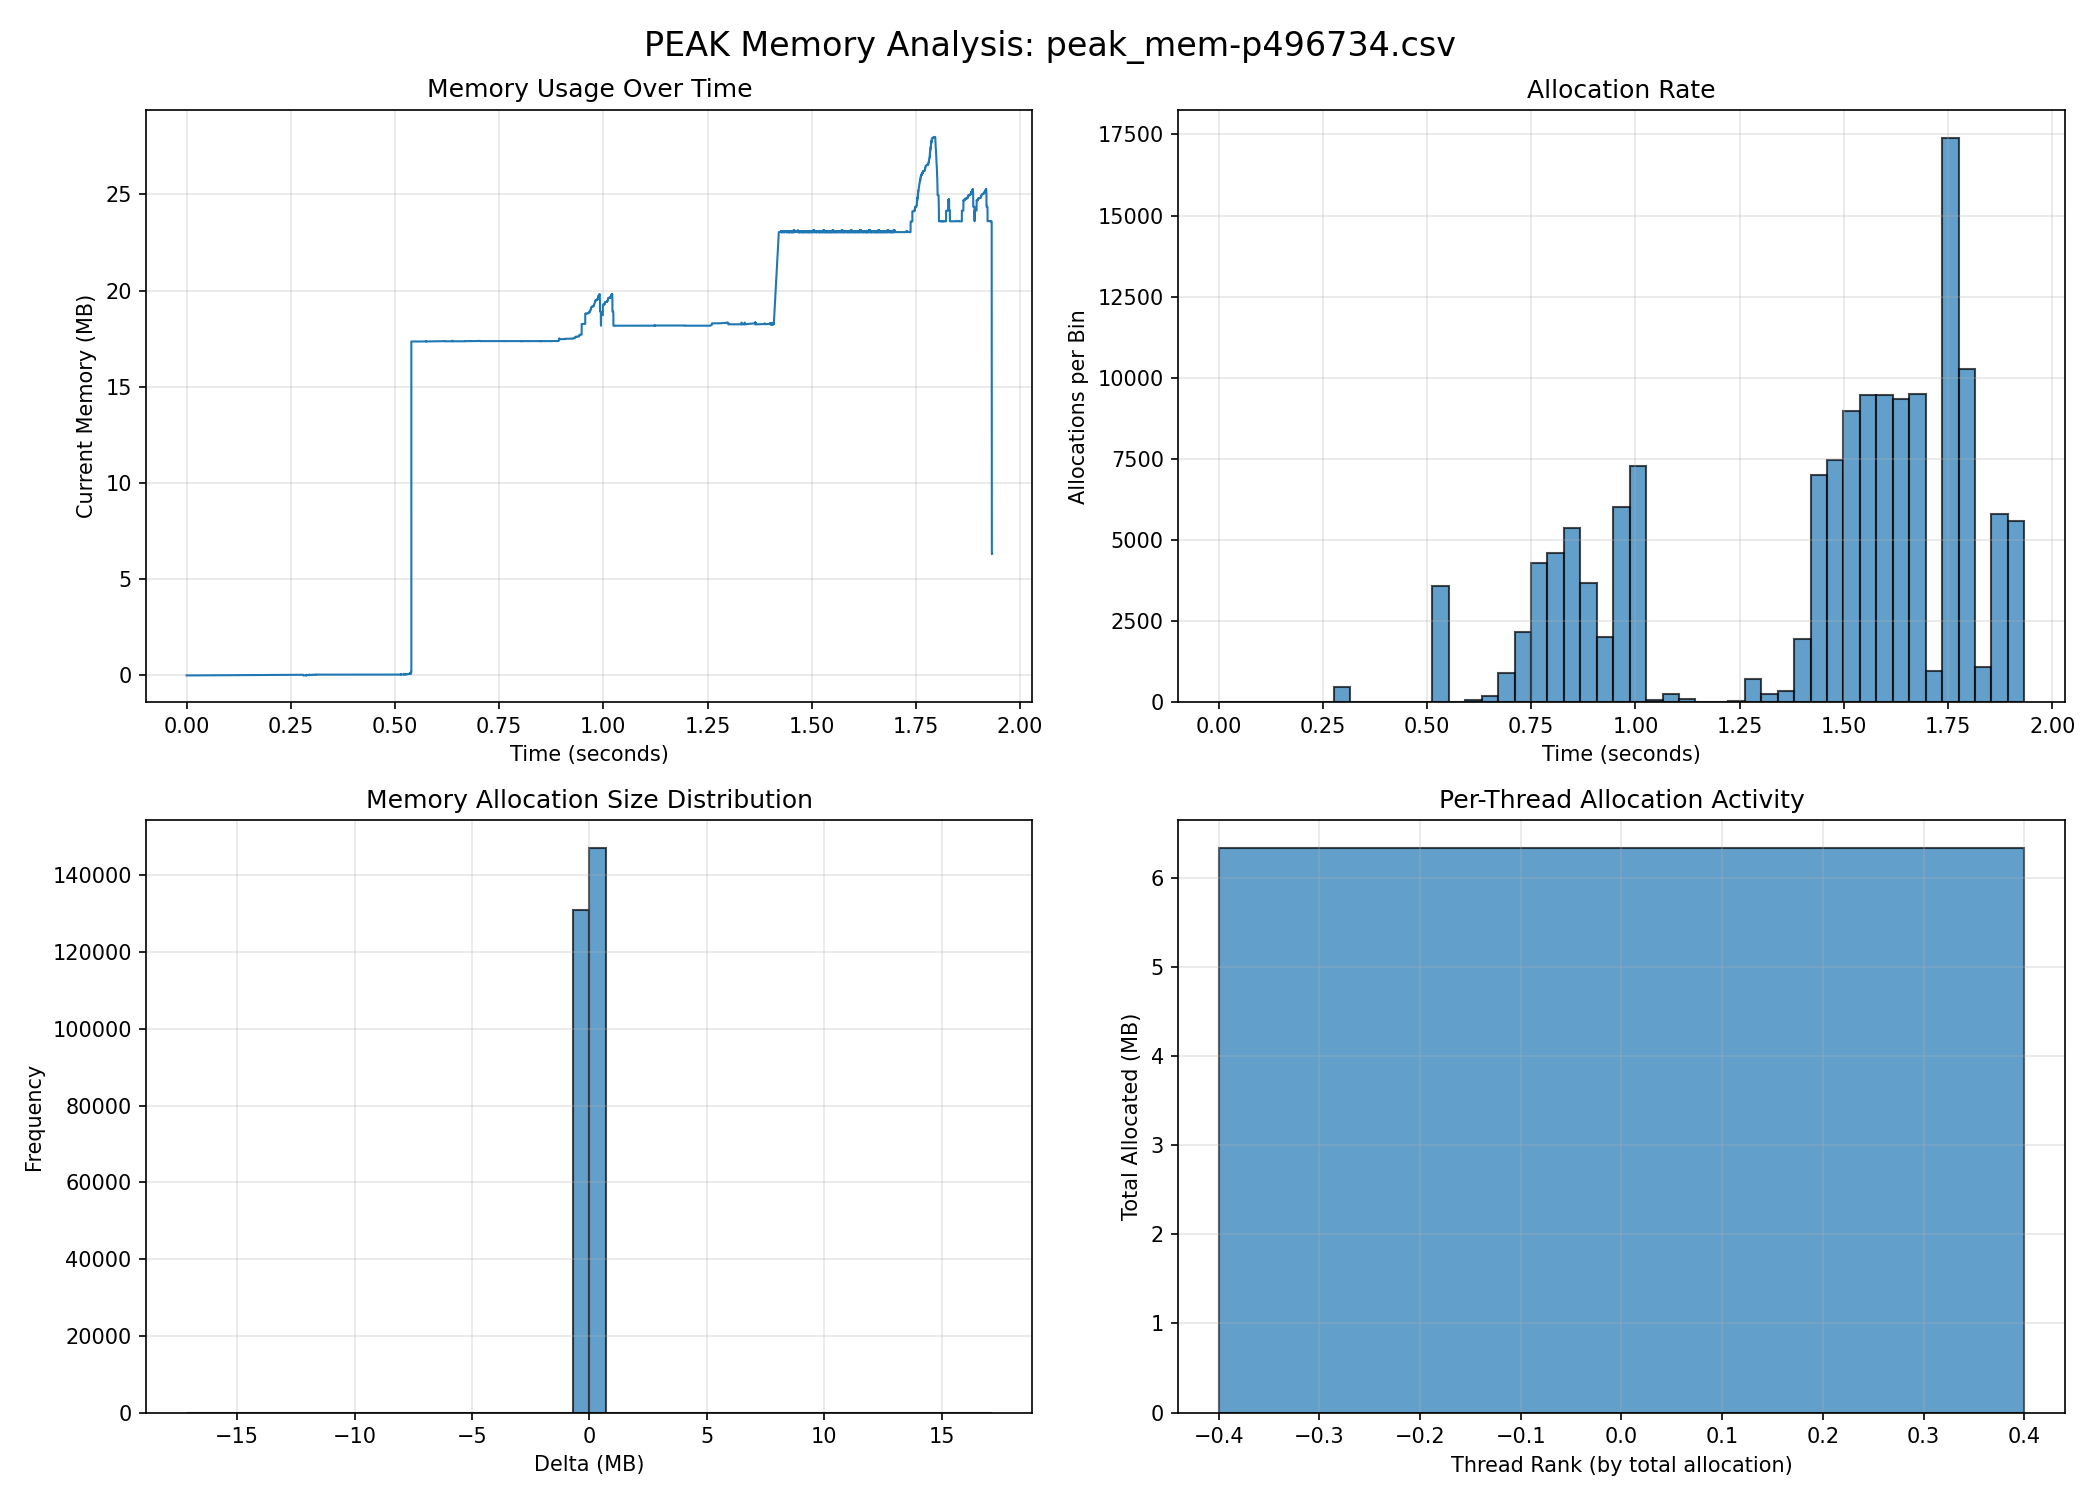
\includegraphics[keepaspectratio]{../abinit/test/peak_mem-p496734_graphs.png}}
\caption{Memory Graph}
\end{figure}

\begin{figure}
\centering
\pandocbounded{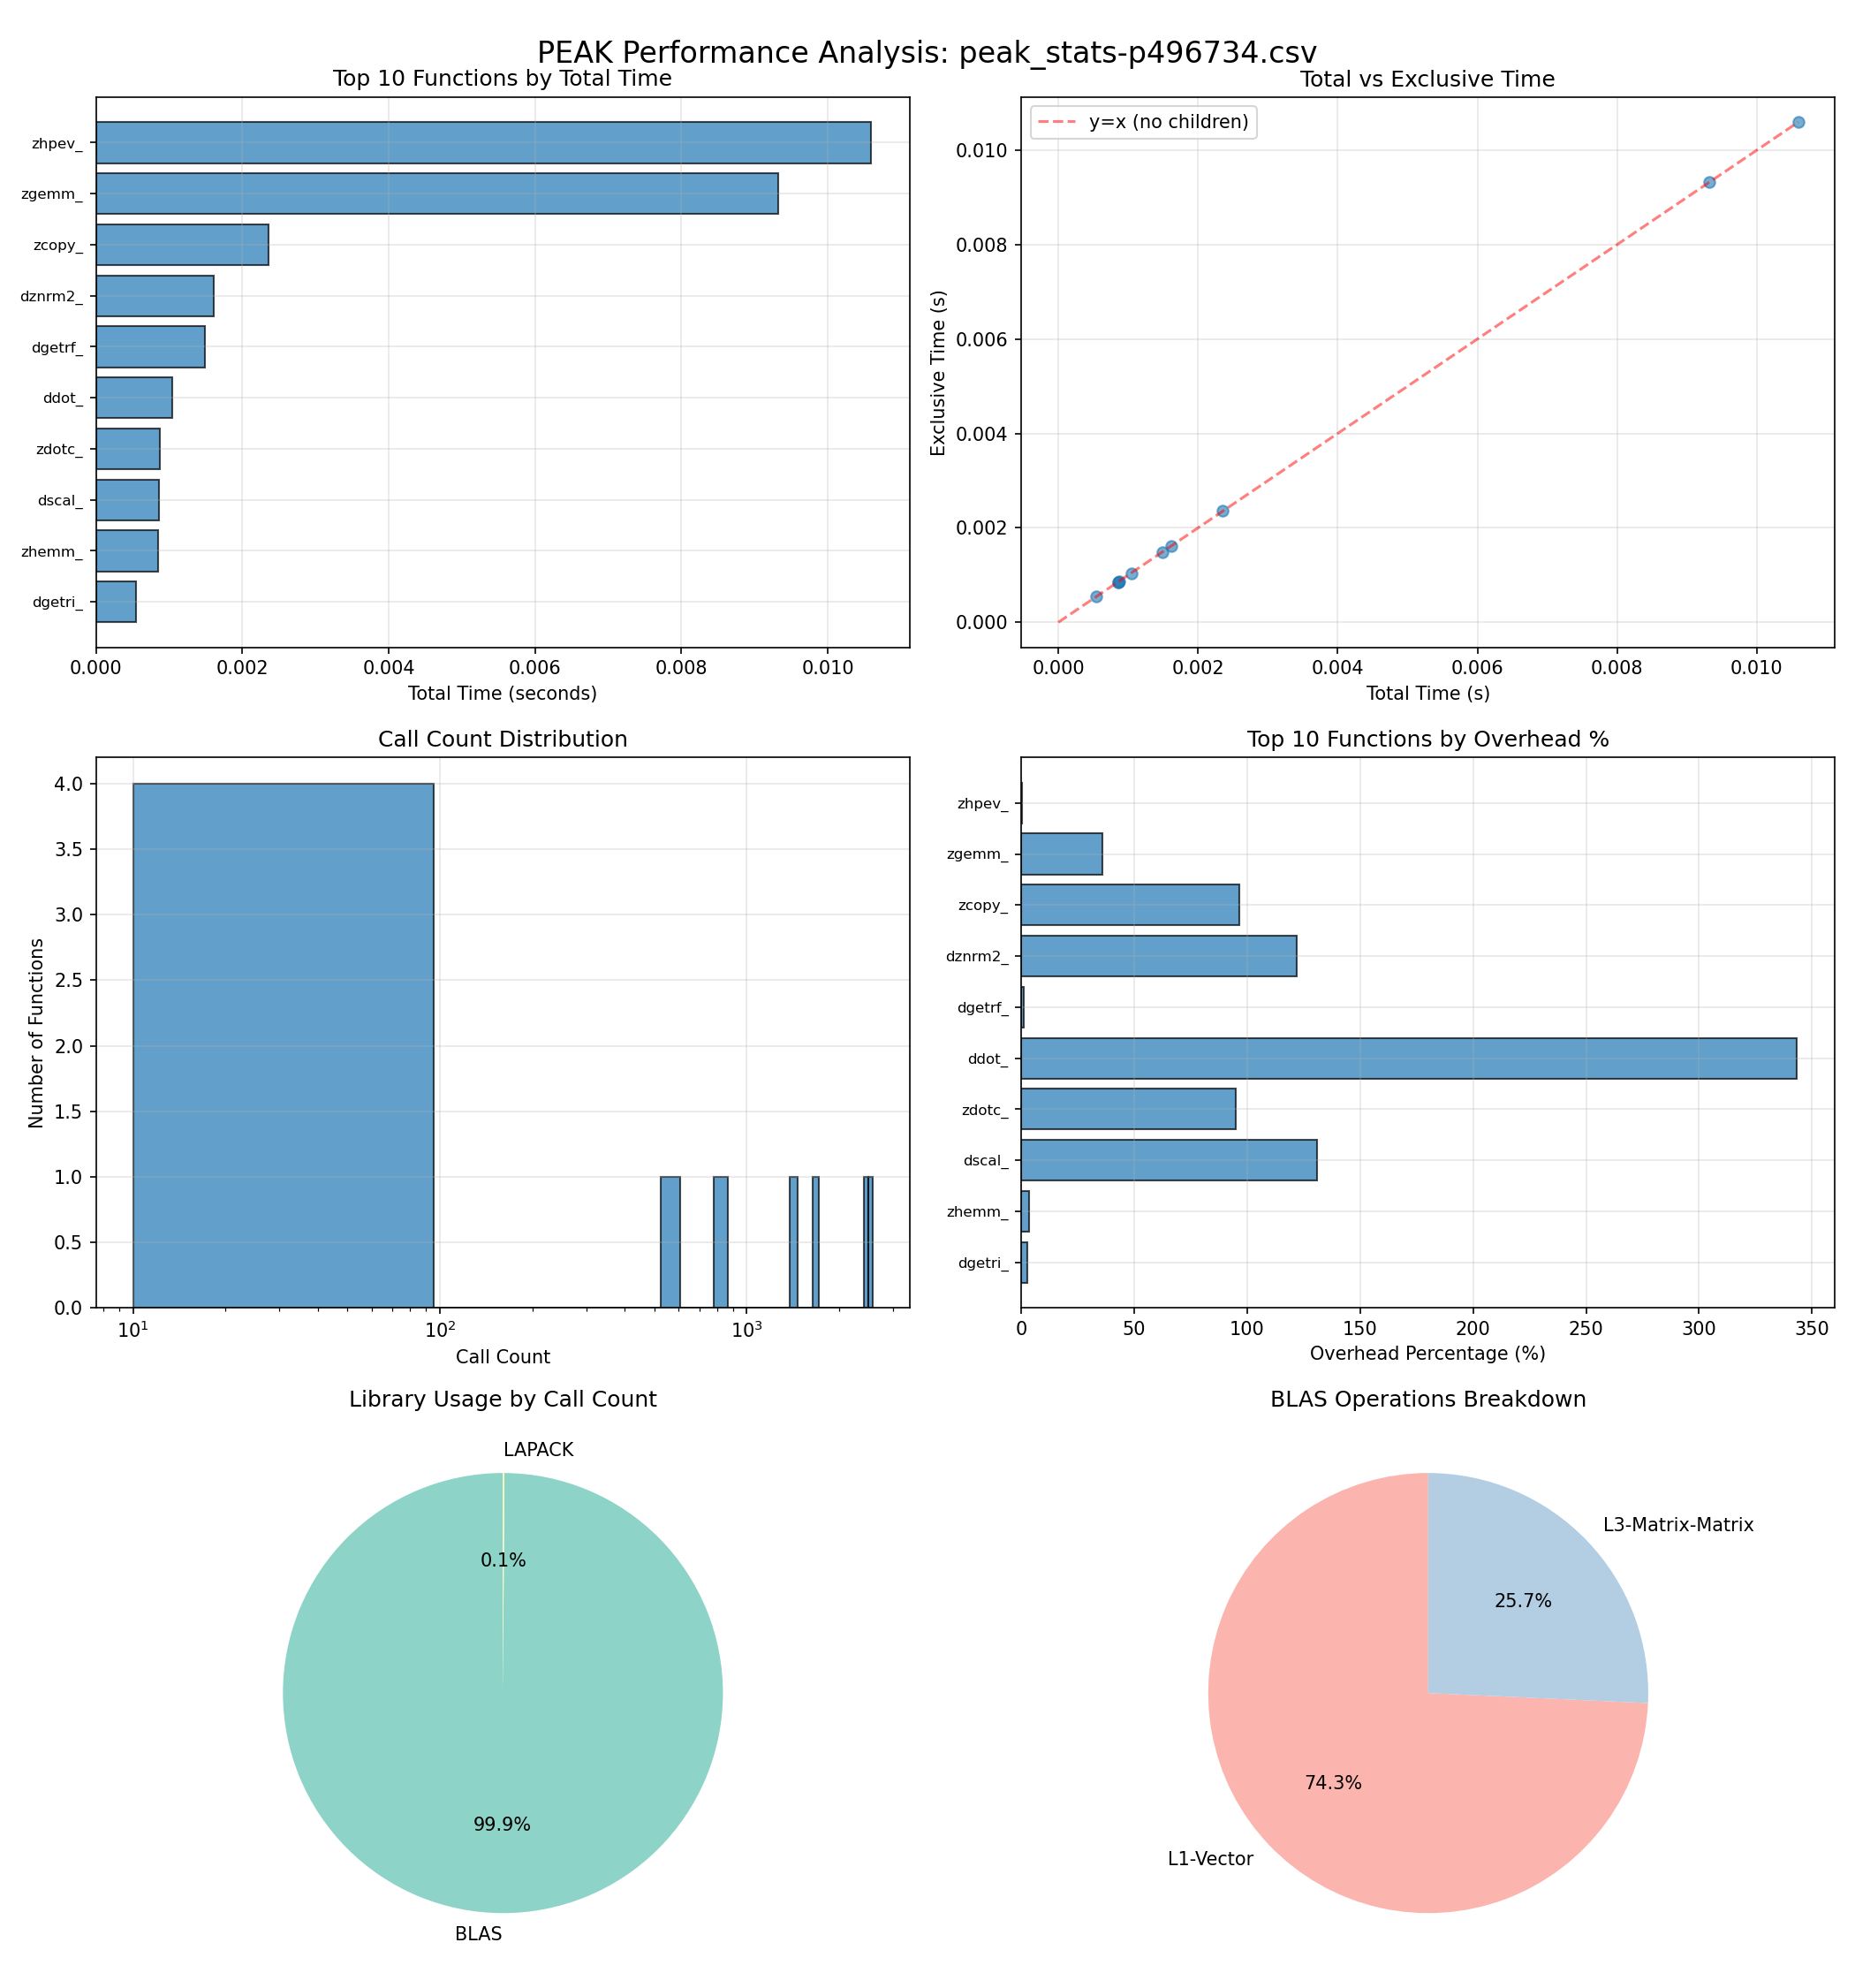
\includegraphics[keepaspectratio]{../abinit/test/peak_stats-p496734_graphs.png}}
\caption{Stat Graph}
\end{figure}

\href{./abinit/test/peak_stats-p496734_library_report.txt}{Library usage
report}

python ../../peak\_analysis\_v2.py peak\_stats-p496734.csv --mem
peak\_mem-p496734.csv

\begin{Shaded}
\begin{Highlighting}[]
\NormalTok{Loading memory log from: peak\_mem{-}p496734.csv}
\NormalTok{Memory graphs saved to: peak\_mem{-}p496734\_graphs.png}

\NormalTok{=== Memory Log Summary ===}
\NormalTok{Total events: 277895}
\NormalTok{Peak memory: 27.99 MB}
\NormalTok{Total allocated: 113.99 MB}
\NormalTok{Total freed: 107.66 MB}
\NormalTok{Unique threads: 1}
\NormalTok{Duration: 1.93 seconds}

\NormalTok{Loading stats log from: peak\_stats{-}p496734.csv}
\NormalTok{Stats graphs saved to: peak\_stats{-}p496734\_graphs.png}
\NormalTok{Library usage report saved to: peak\_stats{-}p496734\_library\_report.txt}

\NormalTok{=== Stats Log Summary ===}
\NormalTok{Total functions profiled: 10}
\NormalTok{Total profiled time: 0.03 seconds}
\NormalTok{Total exclusive time: 0.03 seconds}
\NormalTok{Total overhead: 0.0132 seconds}
\NormalTok{Total calls: 9500}

\NormalTok{=== Top 10 Functions by Total Time ===}
\NormalTok{function  total\_s  exclusive\_s  count}
\NormalTok{  zhpev\_ 0.010592     0.010592     26}
\NormalTok{  zgemm\_ 0.009319     0.009319   2410}
\NormalTok{  zcopy\_ 0.002355     0.002355   1634}
\NormalTok{ dznrm2\_ 0.001615     0.001615   1414}
\NormalTok{ dgetrf\_ 0.001491     0.001491     10}
\NormalTok{   ddot\_ 0.001044     0.001044   2574}
\NormalTok{  zdotc\_ 0.000873     0.000873    596}
\NormalTok{  dscal\_ 0.000856     0.000856    804}
\NormalTok{  zhemm\_ 0.000854     0.000854     22}
\NormalTok{ dgetri\_ 0.000548     0.000548     10}

\NormalTok{=== Library Usage Summary ===}
\NormalTok{Library         Calls        \% Calls    Time (s)}
\NormalTok{{-}{-}{-}{-}{-}{-}{-}{-}{-}{-}{-}{-}{-}{-}{-}{-}{-}{-}{-}{-}{-}{-}{-}{-}{-}{-}{-}{-}{-}{-}{-}{-}{-}{-}{-}{-}{-}{-}{-}{-}{-}{-}{-}{-}{-}{-}{-}{-}{-}{-}{-}{-}{-}{-}{-}}
\NormalTok{BLAS            9454         99.89      0.0169}
\NormalTok{LAPACK          10           0.11       0.0015}

\NormalTok{=== BLAS Breakdown ===}
\NormalTok{  L1{-}Vector            7022         74.28\%}
\NormalTok{  L3{-}Matrix{-}Matrix     2432         25.72\%}
\end{Highlighting}
\end{Shaded}

ABINIT's 0th test seems to very heavily on BLAS for matrix and vector
operations, specifically ddot for vector dot products and zgemm for
matrix multiplication

\paragraph{Methodology}\label{methodology}

\begin{enumerate}
\def\labelenumi{\arabic{enumi}.}
\tightlist
\item
  Build the program
\item
  Wrote a script to run the program
\item
  Ran under idev
\item
  After successful test run, I ran under PEAK with memory, BLAS, LAPACK,
  and FFTW profiling enabled
\item
  Did some basic analysis and visualization of the outputs using a
  python script
\end{enumerate}

\subsubsection{Created a python script to do basic analysis profiling
outputs}\label{created-a-python-script-to-do-basic-analysis-profiling-outputs}

I created a python script to visualize the outputs of PEAK. It graphs
both stat and mem csv's as well as data about target group libraries.

\href{./peak_analysis_v2.py}{peak\_analysis\_v2.py}

\subsubsection{Sorted the top 100 list for actionable and unique
items}\label{sorted-the-top-100-list-for-actionable-and-unique-items}

Removed generic names, interpretors, and consolidated names. Also had AI
write up a blurb for each item so I have a better idea of the programs
use and operations.

\href{./filtered_list.txt}{Filtered top 100 list}
\href{./tacc_hpc_top100_complete_guide.md}{Filtering Report}

\subsubsection{Put together a general research data gathering plan /
guideline / methodology for
myself}\label{put-together-a-general-research-data-gathering-plan-guideline-methodology-for-myself}

\begin{enumerate}
\def\labelenumi{\arabic{enumi}.}
\tightlist
\item
  Build the program
\item
  Use the ABINIT script as a base for a run script
\item
  Test run under idev
\item
  Enable PEAK profiling for memory, BLAS, LAPACK, and FFTW
\item
  Use another script to generate and submit different SLURM jobs in
  order to test affects of Node and MPI scaling. Multiple test inputs
  will also be run.
\item
  Use the python script to organize and visualize the data, grouped by
  the different scalings
\end{enumerate}

\subsubsection{Developed a workflow for
myself}\label{developed-a-workflow-for-myself}

\begin{itemize}
\tightlist
\item
  I'm familiar with git so I'll be using a git repo on both the remote
  and local to keep my data, notes, and scripts organized and available
  to myself and the group.
\end{itemize}

\subsection{What I learned this week}\label{what-i-learned-this-week}

\begin{itemize}
\tightlist
\item
  building on HPC systems
\item
  how to run PEAK on HPC systems and profile for BLAS, LAPACK, and FFTW
\item
  I'm a bit more familiar with the top 100 items now
\end{itemize}

\subsection{Questions / Issues}\label{questions-issues}

\begin{itemize}
\tightlist
\item
  Does my proposed data gathering plan sound good?
\item
  Does the data gathered from ABINIT seem correct?
\end{itemize}

\end{document}
